% Provenance (never printed): see sources/outline_sources.md (Year 2: taphonomy; index fossils;
% facies and fossils as environment markers; reconstructing a palaeoenvironment from a map and a
% section). Taphonomy after Loron (2024); live, dead and fossil assemblages after Tyler and
% Kowalewski (2025); Lagerstaetten after Gaines and others (2024), Mussini and Butterfield
% (2025), Vannier and others (2018), Gerschermann and others (2021) and Rauhut and others
% (2018); zone durations after Al-Suwaidi and others (2022); ichnofacies after Buatois and others
% (2020) and Paz and others (2023); stenohaline groups after McGairy and others (2021) and Saleh
% and others (2022). The Varden column from figdata/shared/region.py; porosities and rates from
% figdata/bachelor-2/palaeoenv.py; exercise and problem values in the Book 4 scratch calculator
% calc/ch20.py. The fossil content given to the Varden units is invented, like the region.
\chapter{Fósiles y paleoambientes}\label{ch:b2:palaeoenvironments}

Sobre una losa de arenisca gris hay tres pistas: el rastro que un trilobites abrió en el fango,
las ondulaciones que dejó una corriente y una madriguera que un gusano excavó y abandonó. Ninguna de ellas es un
animal entero y, sin embargo, juntas dicen que esta ladera fue en otro tiempo el fondo de un mar, lo bastante somero
para que el oleaje lo removiera, lo bastante salado para que vivieran en él trilobites. Los fósiles son los
restos y las huellas de la vida pasada, y los geólogos los leen dos veces: como relojes que datan la roca,
y como testigos del lugar donde se formó. Este capítulo sigue a un ser vivo desde su muerte
hasta el cajón del coleccionista, abre los raros depósitos en los que sobreviven incluso los cuerpos blandos, y después lee
el ambiente de un mar desaparecido, con cifras, en la cobertera de las colinas de Varden.
% ledger: usgs:fossil-record-bulk, loron24:taphonomy

\begin{recall}
\textbf{De los volúmenes escolares}: fósil, molde, contramolde e \omterm{def:b2:palaeoenvironments:fossil-kinds}{icnofósil}; cómo el enterramiento y los minerales
convierten una concha en piedra; la sucesión de los fósiles a lo largo del tiempo. \textbf{Del volumen de primer año}:
las facies sedimentarias y los medios sedimentarios, las turbiditas, los arrecifes y los ooides; las biozonas, los fósiles
guía y los datos de primera aparición; la compactación, la descompactación, la ley de Athy y el espesor sólido
de una capa; el cemento; el espacio de acomodación. \textbf{De capítulos anteriores}: las transgresiones y regresiones,
el nivel del mar a largo plazo y los \omterm{def:b2:phanerozoic-earth:oae}{eventos anóxicos oceánicos} (\cref{ch:b2:phanerozoic-earth}). Cómo
evolucionan las especies, y cómo se clasifican los animales y las plantas, corresponde a los libros de biología.
\end{recall}

\section{De la muerte al fósil}\label{sec:b2:palaeoenvironments:taphonomy}

La mayoría de los seres vivos no dejan nada tras de sí. Las bacterias y los carroñeros consumen las partes blandas en
días o años, las corrientes rompen y dispersan las duras, y los ácidos de los suelos y de las aguas intersticiales
disuelven lo que queda. Un fósil es lo que sobrevive a todo esto, y sobrevive además al enterramiento,
al calentamiento y al levantamiento de la roca que lo contiene.

\begin{definition}[Tafonomía; potencial de preservación]\label{def:b2:palaeoenvironments:taphonomy}
La \emph{tafonomía}\index{tafonomia@tafonomía} es el estudio de lo que les ocurre a los restos de un organismo
desde su muerte hasta su descubrimiento como fósil: descomposición, carroñeo, transporte, enterramiento y los
cambios químicos de la diagénesis. El \emph{potencial de preservación}\index{potencial de preservacion@potencial de preservación}
de un organismo, o de una de sus partes, es la probabilidad de que pase por estas etapas
y sobreviva en la roca.
\end{definition}
% ledger: loron24:taphonomy

Cada etapa quita algo, añade algo o cambia algo. La descomposición y el carroñeo eliminan los
tejidos blandos; los minerales del agua intersticial rellenan los poros de un hueso o sustituyen el aragonito de una
concha, añadiendo materia que el animal nunca tuvo; el calentamiento altera las moléculas orgánicas que quedan.
Loron clasifica todos estos cambios post mortem en tres clases, ganancia, pérdida y alteración, y
los escribe como una sola ecuación para el cambio de cualquier rasgo medible entre un organismo y su
fósil. La figura siguiente recorre las etapas y lo que cada una se lleva.
% ledger: loron24:taphonomy

\begin{omfigure}
\centering
\begin{tikzpicture}[font=\scriptsize, x=1cm, y=1cm,
  stage/.style={draw=black!60, fill=omSea!12, rounded corners=2pt, align=center,
    text width=2.05cm, minimum height=1.25cm, inner sep=2pt},
  loss/.style={align=center, text width=2.05cm, text=omThm!80!black}]
\node[stage] (a) at (0,0) {\textbf{muerte}\\una comunidad\\viva};
\node[stage] (b) at (2.75,0) {\textbf{degradación}\\\textbf{y carroñeo}\\en el fondo};
\node[stage] (c) at (5.5,0) {\textbf{transporte}\\las corrientes\\clasifican y rompen};
\node[stage] (d) at (8.25,0) {\makebox[\linewidth]{\textbf{enterramiento}}\\bajo la capa\\activa};
\node[stage] (e) at (11,0) {\textbf{diagénesis}\\compactación,\\sustitución};
\node[stage] (f) at (13.75,0) {\textbf{exhumación}\\y\\recolección};
\foreach \u/\v in {a/b, b/c, c/d, d/e, e/f} {\draw[-{Stealth[length=2mm]}, black!70] (\u) -- (\v);}
\node[loss, anchor=north] at (2.75,-0.8) {tejido blando perdido;\\esqueletos desarticulados};
\node[loss, anchor=north] at (5.5,-0.8) {partes ligeras arrastradas,\\conchas rotas};
\node[loss, anchor=north] at (8.25,-0.8) {enterramiento lento: más\\tiempo para las pérdidas};
\node[loss, anchor=north] at (11,-0.8) {aragonito disuelto,\\minerales añadidos};
\node[loss, anchor=north] at (13.75,-0.8) {erosionado,\\o nunca hallado};
\end{tikzpicture}
\par\smallskip{\small El recorrido tafonómico de una comunidad viva a una colección, con lo que
cada etapa elimina o cambia. El enterramiento es el punto de inflexión: antes, los restos están expuestos a
todas las pérdidas; después, solo actúan sobre ellos la diagénesis y la erosión.}
\end{omfigure}
% ledger: loron24:taphonomy

Los volúmenes escolares llamaban fósil a cualquier resto o huella de vida pasada conservado en una roca. Las dos clases
se comportan de forma tan distinta en la roca que merecen nombres propios.

\begin{definition}[Fósil corporal; icnofósil]\label{def:b2:palaeoenvironments:fossil-kinds}
Un \emph{fósil corporal}\index{fosil corporal@fósil corporal} es una parte del cuerpo de un organismo, o el molde o contramolde
de esa parte: una concha, un hueso, un diente, una hoja y, en depósitos raros, un tejido blando. Un
\emph{icnofósil}\index{icnofosil@icnofósil} es una estructura que un organismo hizo con su actividad en un
sedimento o una roca, o sobre ellos: una pisada, un rastro, una madriguera, una perforación, una pauta de alimentación.
\end{definition}

Un \omterm{def:b2:palaeoenvironments:fossil-kinds}{icnofósil} forma parte del sedimento en el que se excavó: una corriente que lo moviera lo destruiría.
Registra por tanto las condiciones del lugar exacto donde vivía su autor, cosa que una concha,
fácil de arrastrar por el fondo, no siempre hace. Los \omterm{def:b2:palaeoenvironments:fossil-kinds}{icnofósiles} se nombran como los organismos, con un
género y una especie, pero el nombre describe la estructura, no el animal: la misma madriguera puede
excavarla varias clases de animales, y un solo animal puede dejar varias clases de huella.

\subsection*{Enterramiento frente a destrucción}

La carrera entre el enterramiento y la destrucción puede plasmarse en un modelo sencillo. Los restos que yacen en el
fondo se destruyen a un ritmo constante $k$, la probabilidad por unidad de tiempo de que sean comidos,
rotos o disueltos; están a salvo una vez que los cubre un espesor $h$ de sedimento; y el
sedimento se acumula a la velocidad $s$.

\begin{proposition}[Enterramiento antes de la destrucción]\label{prop:b2:palaeoenvironments:burial}
Con estas hipótesis, la probabilidad de que un resto llegue a estar a salvo es
\[
  P = e^{-kh/s}.
\]
Depende de las tres magnitudes solo a través de la razón entre el tiempo hasta el enterramiento, $h/s$, y el
tiempo medio de supervivencia en el fondo, $1/k$.
\end{proposition}

\begin{proof}
El resto necesita el tiempo $T = h/s$ para quedar cubierto por el espesor $h$. Con un ritmo de
destrucción constante $k$, la probabilidad $p(t)$ de sobrevivir hasta el tiempo $t$ cumple $p' = -kp$, $p(0) =
1$, de modo que $p(t) = e^{-kt}$; en $t = T$ esto da $e^{-kh/s}$.
\end{proof}

\begin{example}[Una concha en un fondo tranquilo]\label{ex:b2:palaeoenvironments:shell}
Supóngase que una concha sobrevive en el fondo 20 años de media, $k = \qty{0.05}{yr^{-1}}$, y que está
a salvo bajo $h = \qty{0.1}{m}$ de fango. Con $s = \qty{1}{mm.yr^{-1}}$ el tiempo hasta el enterramiento es de 100
años y $P = e^{-5} = 0.0067$: sobrevive menos de una concha de cada cien. Con
\qty{1}{cm.yr^{-1}}, $P = e^{-0.5} = 0.61$. Una tormenta que vierte \qty{0.3}{m} de arena en un día
lo entierra todo de una vez, y entonces $P$ es cercana a uno. Las cifras son supuestas, pero la lección
no: los fósiles se concentran donde el sedimento llega deprisa o en capas repentinas.
\end{example}

El modelo muestra también por qué el registro está sesgado. Un gusano de cuerpo blando, cuyo tiempo medio de supervivencia en
el fondo es de días y no de decenios, tiene un valor de $k$ cientos de veces mayor que una concha
gruesa, y por tanto una probabilidad exponencialmente menor. La mayor parte del registro fósil está formada por animales
con concha y por restos microscópicos. Tyler y Kowalewski midieron cuánto pierde una comunidad en
su camino hacia la roca. En 51 estaciones de un fondo marino costero contaron 135 especies vivas de
invertebrados, 150 especies entre las conchas y los esqueletos que yacían muertos en el fondo, y 112 que
tienen además registro fósil. Los muertos superan a los vivos porque las conchas del fondo se acumularon
a lo largo de muchos años, procedentes de animales que ya no viven allí. Los detritívoros y los carnívoros, en su mayoría
de cuerpo blando, son los que menos probabilidades tienen de conservarse; aun así, los principales grupos ecológicos de la
comunidad viva se encontraron todos entre los muertos.
% ledger: usgs:fossil-record-bulk, tyler25:live-dead, tyler25:soft-bodied

\section{Ventanas de preservación excepcional}\label{sec:b2:palaeoenvironments:lagerstatten}

\begin{definition}[Lagerstätte]\label{def:b2:palaeoenvironments:lagerstatte}
Un \emph{Lagerstätte}\index{Lagerstätte} (plural Lagerstätten) es un depósito sedimentario que
conserva fósiles de calidad excepcional, en particular los tejidos blandos, no biomineralizados, que
la descomposición destruye casi en todas partes; un depósito así se llama también Konservat-Lagerstätte.
\end{definition}
% ledger: gaines24:konservat

Los Lagerstätten son raros, pero buena parte de lo que se sabe de los animales de cuerpo blando procede de ellos, y
la primera gran radiación de los animales, en el Cámbrico, se entiende mejor gracias a ellos.
% ledger: gaines24:konservat

\subsection*{El esquisto de Burgess}

En 1909 Charles Walcott dibujó en su libreta de campo un pequeño artrópodo que había encontrado en el esquisto de
Burgess, en la Columbia Británica. Más tarde recogió cientos de
ejemplares de él, \emph{Waptia}, en un único intervalo de unos \qty{2}{m} de espesor, el Phyllopod
Bed; su descripción moderna se basa en más de 1800 ejemplares conservados en dos museos. El esquisto de
Burgess, de unos 508 millones de años, se depositó en aguas más profundas, frente a un escarpe submarino
abrupto. Entre sus fósiles hay animales sin concha, conservados como películas aplastadas de carbono,
a menudo cuerpos enteros. Esa preservación está ligada al enterramiento en fangos pobres en oxígeno que los animales no
bioturbaban y que las corrientes no removían: las pérdidas de la figura anterior se detuvieron de inmediato.
% ledger: vannier18:waptia, mussini25:burgess

\begin{omfigure}
\centering
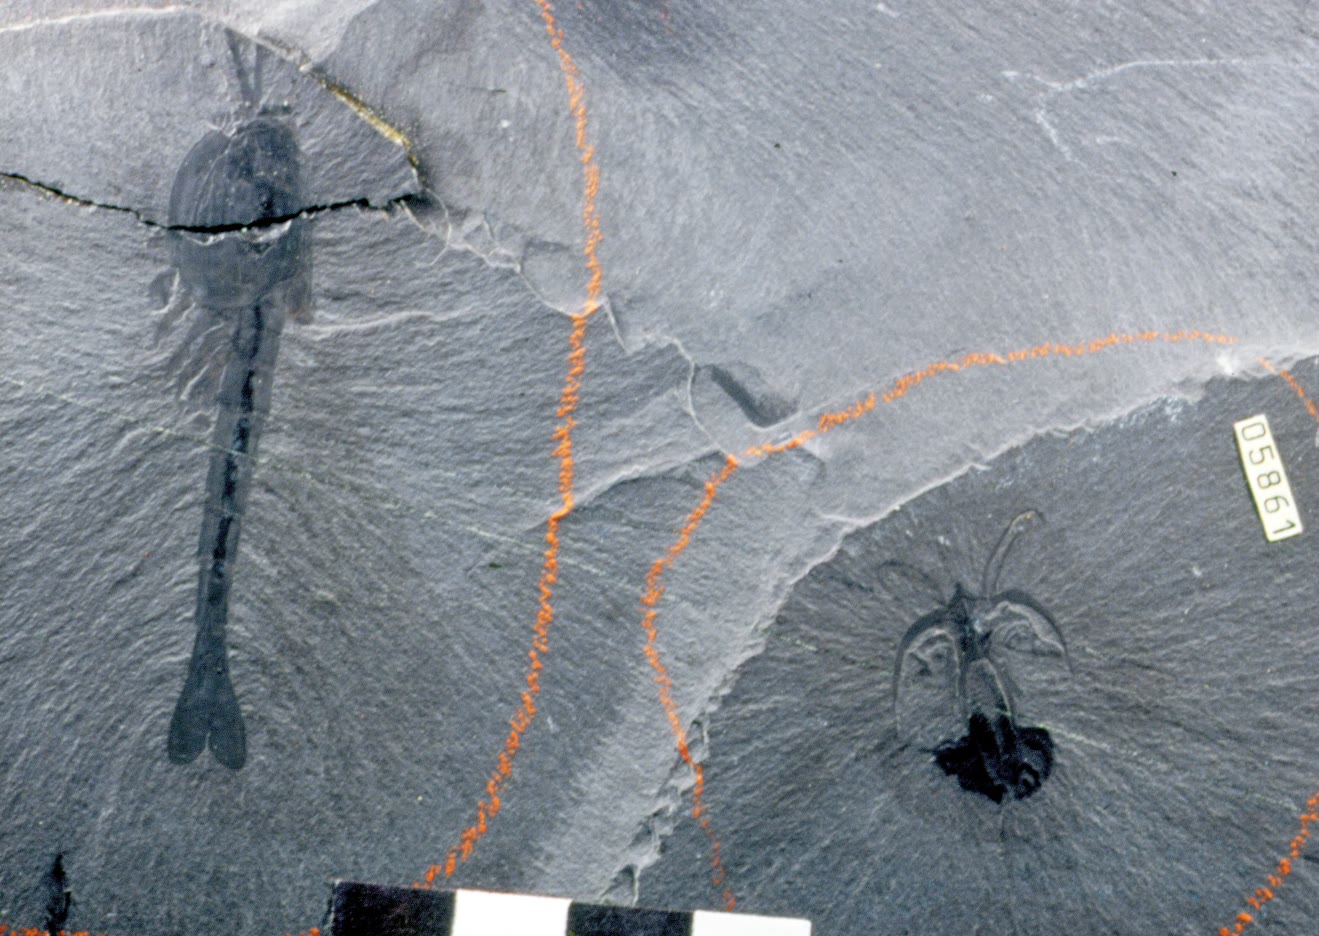
\includegraphics[width=0.72\linewidth]{images/book4/b2-20-burgess-waptia-marrella.jpg}
\par\smallskip{\small Dos artrópodos del esquisto de Burgess, conservados como películas oscuras de carbono:
\emph{Waptia} (izquierda) y \emph{Marrella} (derecha). (James
St.~John, CC~BY~2.0, a través de Wikimedia Commons.)}
\end{omfigure}
% ledger: mussini25:burgess

\subsection*{Solnhofen}

Las calizas de grano fino de Solnhofen y Eichstätt, en Baviera, se depositaron en lagunas
a comienzos del Titoniense, la última edad del Jurásico, que empezó hace \qty{149.2}{Ma}. Son
la localidad tipo de doce ejemplares de \emph{Archaeopteryx}, de numerosos pterosaurios y de peces
cuyos tejidos blandos e incluso patrones de color sobreviven. Los fósiles son allí raros, pero su
preservación es extraordinaria. Se han propuesto varias condiciones, quizá actuando juntas:
aguas de fondo unas tres veces más saladas que el agua de mar o muy alcalinas, que frenan la descomposición
bacteriana; tapetes bacterianos que sellaban los cadáveres; aguas de fondo sin oxígeno, que mantenían
alejados a los carroñeros; y tormentas que removían el fango calcáreo y enterraban deprisa los cadáveres. Cada
una de ellas alarga el tiempo de supervivencia $1/k$ o acorta el tiempo hasta el enterramiento $h/s$.
% ledger: gerschermann21:solnhofen, rauhut18:archaeopteryx, ics4:jurassic-stages

\begin{omfigure}
\centering
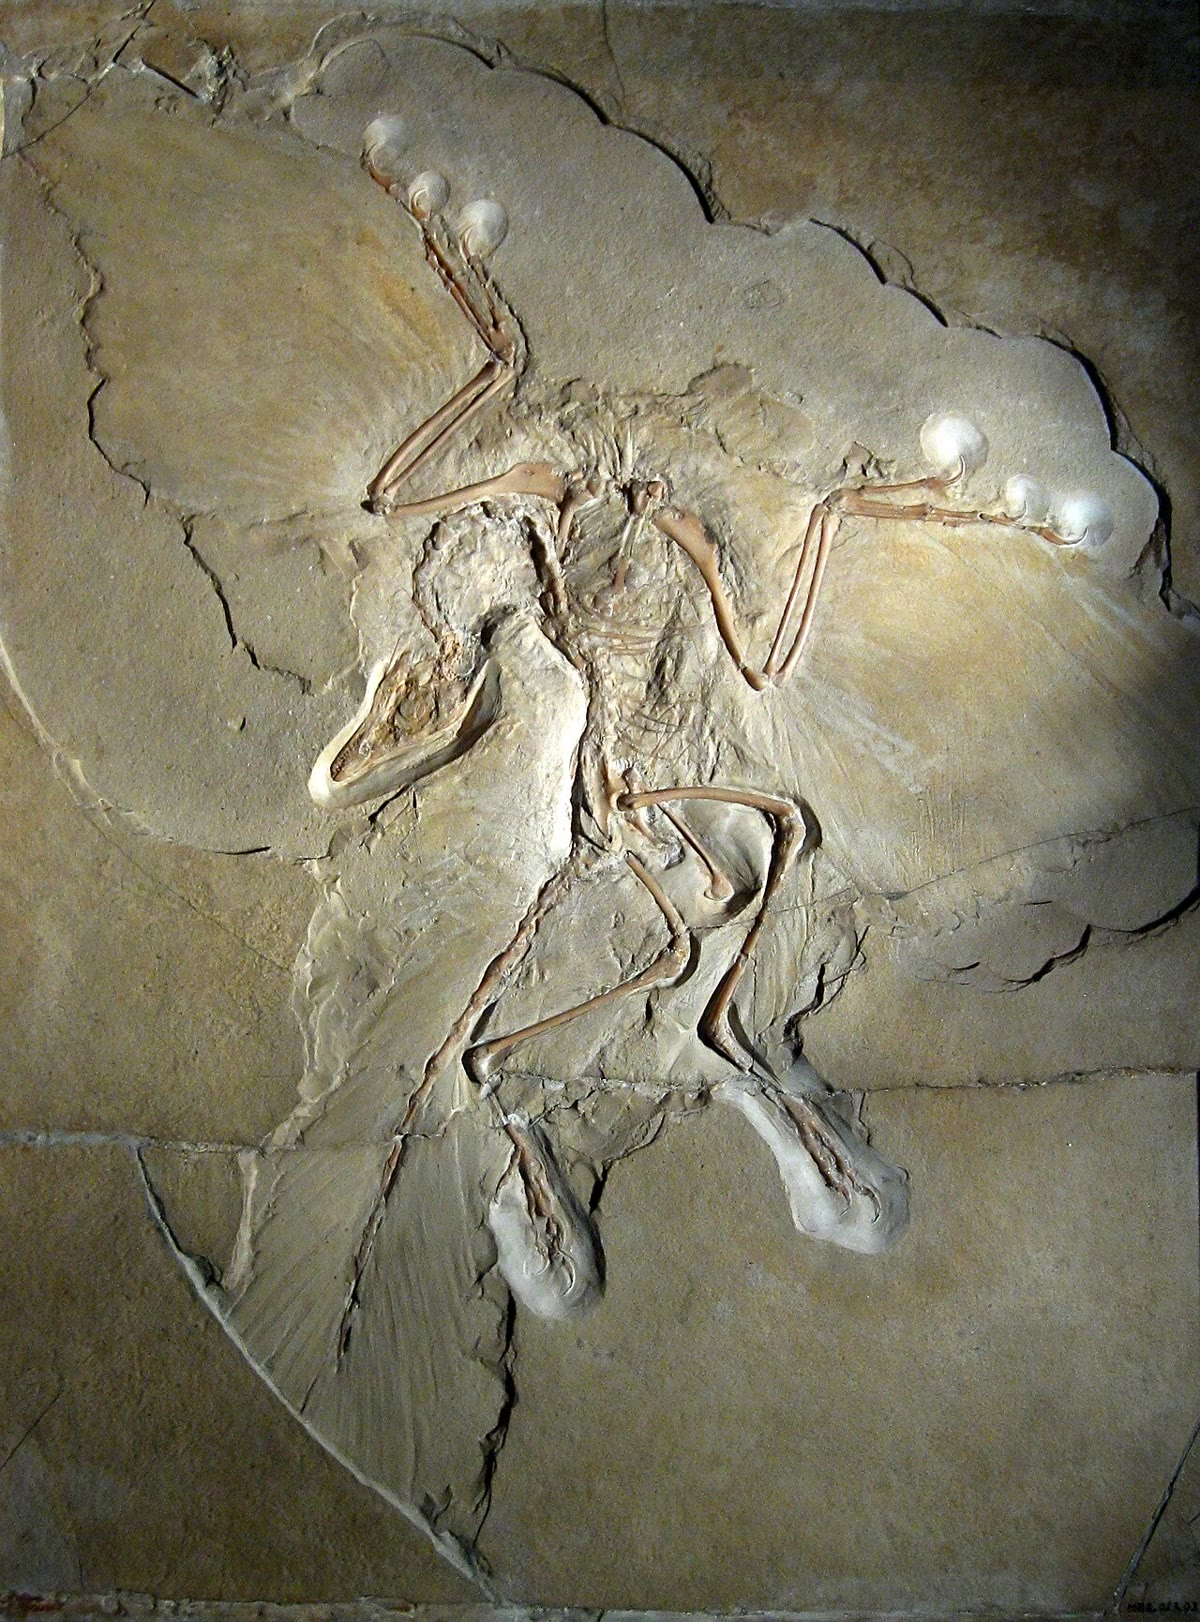
\includegraphics[width=0.5\linewidth]{images/book4/b2-20-archaeopteryx-berlin.jpg}
\par\smallskip{\small El ejemplar de Berlín de \emph{Archaeopteryx}, de las calizas de
Solnhofen: los huesos y las impresiones de las plumas de las alas y la cola. (H.~Raab, CC~BY-SA~3.0,
a través de Wikimedia Commons.)}
\end{omfigure}
% ledger: rauhut18:archaeopteryx, gerschermann21:solnhofen

\subsection*{Los fósiles como relojes}

El volumen de primer año construyó la biozona, un conjunto de estratos definido por sus fósiles, y el fósil
guía que la reconoce. ¿Qué precisión tiene ese reloj? Una zona de ammonites jurásica puede durar
alrededor de un millón de años: la primera zona del Toarciense, datada con edades uranio--plomo de capas de ceniza de
Argentina, abarca de 183.73 a \qty{182.77}{Ma}. Las zonas se dividen en horizontes, y en el Jurásico
Superior un horizonte de ammonites dura en promedio \qty{165}{kyr}. Todos los esqueletos de
\emph{Archaeopteryx} proceden de una sola zona que contiene cinco horizontes, de modo que el ave se conoce a lo largo de
unos 0.7 a 1 millón de años. Los fósiles, sin embargo, solo dan un orden; las edades en años proceden
de capas de ceniza datadas por uranio y plomo, y de ciclos sedimentarios. Las mismas capas de ceniza sitúan la base del Toarciense en $183.73$, con una incertidumbre de
$+0.35$ y \qty{-0.50}{Myr}, donde la tabla internacional da \qty{184.2}{Ma}.
% ledger: alsuwaidi22:toarcian, rauhut18:archaeopteryx, ics4:jurassic-stages

\section{Los fósiles como testigos del ambiente}\label{sec:b2:palaeoenvironments:environment}

Para leer un ambiente en un fósil, un geólogo supone que el organismo vivía donde viven sus parientes
actuales, y que los procesos que actúan hoy sobre el sedimento actuaban entonces de la misma manera.

\begin{definition}[Actualismo]\label{def:b2:palaeoenvironments:actualism}
El \emph{actualismo}\index{actualismo} es el método que interpreta los registros geológicos del pasado mediante los
procesos, y las relaciones entre los organismos y su ambiente, que pueden observarse hoy.
\end{definition}

En 1830 Charles Lyell dio al primer volumen de sus \emph{Principles of Geology} el subtítulo «un
intento de explicar los cambios pasados de la superficie de la Tierra por referencia a causas que actúan
en la actualidad». El método tiene límites. Muchos grupos están extinguidos, y su modo de vida debe
deducirse de su forma y del sedimento que los rodea; y un ambiente del pasado puede
no tener un equivalente exacto hoy.
% ledger: lyell1830:title

\begin{definition}[Paleoambiente]\label{def:b2:palaeoenvironments:palaeoenvironment}
Un \emph{paleoambiente}\index{paleoambiente} es el conjunto de condiciones físicas, químicas y
biológicas que reinaban donde y cuando se formó una roca: el marco, la profundidad y la
energía del agua, su salinidad, su temperatura y su oxígeno, la naturaleza del fondo y la vida
sobre él.
\end{definition}

\subsection*{¿Dónde vivía el fósil?}

La primera pregunta es si los fósiles vivieron donde yacen.

\begin{definition}[Asociaciones de vida y de muerte; fósiles autóctonos y alóctonos]\label{def:b2:palaeoenvironments:assemblages}
Una \emph{asociación de vida}\index{asociacion de vida@asociación de vida} es un grupo de fósiles de organismos que vivieron
juntos, conservados donde y como vivían; una \emph{asociación de muerte}\index{asociacion de muerte@asociación de muerte} es
un grupo de restos reunidos tras la muerte, que puede mezclar organismos de lugares distintos
y de épocas distintas. Un fósil es \emph{autóctono}\index{fosil autoctono@fósil autóctono} si se
conserva donde vivía el organismo, y \emph{alóctono}\index{fosil aloctono@fósil alóctono} si fue
transportado desde otro lugar antes del enterramiento.
\end{definition}

Las pistas son las del transporte. Conchas todavía cerradas, un coral o un bivalvo excavador en su
posición de crecimiento, espinas delicadas intactas, todas las edades de una población presentes: los fósiles son
probablemente \omterm{def:b2:palaeoenvironments:assemblages}{autóctonos}. Valvas sueltas clasificadas por tamaño, fragmentos desgastados y rotos, conchas
concentradas en la base de una capa granoclasificada: fueron transportados. Una \omterm{def:b2:palaeoenvironments:assemblages}{asociación de muerte} de conchas, como
la del fondo costero anterior, conserva aún la mayor parte de la comunidad, pero reúne muchos años
de ella en una sola capa: sus fósiles están promediados en el tiempo.
% ledger: tyler25:live-dead

\subsection*{Salinidad y oxígeno}

Algunos animales solo toleran la salinidad del mar abierto: se llaman estenohalinos. Los equinodermos,
los cefalópodos, los corales y, en el Paleozoico, los trilobites son grupos estenohalinos típicos; su
presencia habla a favor de un agua de mar normal, y su ausencia en una fauna rica puede hablar en contra.
Los depósitos de un estuario silúrico de Vietnam contienen restos vegetales, huesos de peces, bivalvos, gasterópodos
y ostrácodos, pero ninguno de esos grupos. Los equinodermos faltan también en la biota de Chengjiang,
un \omterm{def:b2:palaeoenvironments:lagerstatte}{Lagerstätte} de unos 518 millones de años, aunque aparecen en Lagerstätten de mar abierto del
Cámbrico: los animales de Chengjiang vivían frente a un delta, donde el agua dulce hacía fluctuar la salinidad.
% ledger: mcgairy21:stenohaline, saleh22:echinoderms, saleh22:age

El oxígeno deja su marca a través de los organismos excavadores. Donde el agua del fondo tiene oxígeno, los animales mezclan el
sedimento y destruyen su laminación fina; donde no lo tiene, las láminas sobreviven, faltan las madrigueras
y se forma pirita, como en las lutitas negras de los \omterm{def:b2:phanerozoic-earth:oae}{eventos anóxicos oceánicos} del
\cref{ch:b2:phanerozoic-earth}. La misma falta de excavadores protegió los cadáveres del esquisto de
Burgess.
% ledger: mussini25:burgess

\subsection*{Icnofacies}

Los \omterm{def:b2:palaeoenvironments:fossil-kinds}{icnofósiles} son los mejores testigos del fondo, porque no se movieron. Sus autores
responden a la energía del agua, a la firmeza del fondo, al alimento y al oxígeno, y las
mismas asociaciones de huellas se repiten a lo largo del Fanerozoico.

\begin{definition}[Icnofacies]\label{def:b2:palaeoenvironments:ichnofacies}
Una \emph{icnofacies}\index{icnofacies} es una asociación recurrente de \omterm{def:b2:palaeoenvironments:fossil-kinds}{icnofósiles} que
refleja un conjunto de condiciones ambientales; recibe el nombre de una huella característica.
\end{definition}

A lo largo de un perfil marino, de la costa a la cuenca profunda, se suceden cuatro \omterm{def:b2:palaeoenvironments:ichnofacies}{icnofacies} marinas
(figura siguiente). La \omterm{def:b2:palaeoenvironments:ichnofacies}{icnofacies} de \emph{Skolithos}, dominada por madrigueras de habitación verticales, cilíndricas o
en U de organismos suspensívoros, con pocas huellas horizontales, es típica de la
zona intermareal y de la playa sumergida. La \omterm{def:b2:palaeoenvironments:ichnofacies}{icnofacies} de \emph{Cruziana}, dominada por las madrigueras de
sedimentívoros, con las huellas de ramoneadores, carnívoros y suspensívoros, es típica de la
plataforma externa: el fondo entre el nivel de base del oleaje de buen tiempo, la profundidad por encima de la cual el oleaje ordinario remueve
el sedimento, y el nivel de base del oleaje de tormenta, al que solo llegan las olas de tormenta. La \omterm{def:b2:palaeoenvironments:ichnofacies}{icnofacies} de \emph{Zoophycos},
llamada así por una madriguera que remueve el sedimento en láminas helicoidales alrededor de un eje
central, es típica de la plataforma por debajo del nivel de base del oleaje de tormenta y del talud. La \omterm{def:b2:palaeoenvironments:ichnofacies}{icnofacies} de \emph{Nereites},
con sus madrigueras regulares en meandros, en espiral y en red, interpretadas como las trampas y
los huertos de animales que encontraban poco alimento, es típica del mar profundo más allá del borde de la plataforma. En
las bahías y estuarios salobres, la regla es una \omterm{def:b2:palaeoenvironments:ichnofacies}{icnofacies} de Cruziana con pocas especies.
% ledger: buatois20:ichnofacies, miguez21:ichnofacies, zhang15:zoophycos, buatois25:graphoglyptids, paz23:nereites

\begin{omfigure}
\centering
\begin{tikzpicture}[font=\scriptsize, x=1cm, y=1cm]
% sea and floor (schematic, not to scale)
\fill[omSea!20] (0.6,0) -- (14,0) -- (14,-3.6) -- (11.2,-3.6) -- (9.6,-1.9) -- (6.2,-1.5)
  -- (3.2,-0.9) -- (1.2,-0.15) -- cycle;
\fill[omLithSand!45] (0,0.25) -- (0.6,0) -- (1.2,-0.15) -- (3.2,-0.9) -- (6.2,-1.5)
  -- (9.6,-1.9) -- (11.2,-3.6) -- (14,-3.6) -- (14,-4.3) -- (0,-4.3) -- cycle;
\draw[black!70, line width=0.6pt] (0,0.25) -- (0.6,0) -- (1.2,-0.15) -- (3.2,-0.9) -- (6.2,-1.5)
  -- (9.6,-1.9) -- (11.2,-3.6) -- (14,-3.6);
\draw[omSea!80!black, line width=0.6pt] (0.6,0) -- (14,0);
\node[anchor=south east, omSea!80!black] at (14,0) {nivel del mar};
% wave bases
\draw[dashed, black!60] (2.133,-0.5) -- (14,-0.5) node[anchor=south east, black!70] {nivel de base del oleaje de buen tiempo};
\draw[dashed, black!60] (4.7,-1.2) -- (14,-1.2) node[anchor=south east, black!70] {nivel de base del oleaje de tormenta};
% zone labels
\node[align=center] at (1.9,0.55) {intermareal,\\playa sumergida};
\node[align=center] at (4.6,0.55) {plataforma externa};
\node[align=center] at (8.0,0.55) {plataforma};
\node[align=center] at (10.5,0.55) {talud};
\node[align=center] at (12.7,0.55) {cuenca};
% Skolithos: vertical tubes
\foreach \x in {1.75,1.95,2.15,2.35} {\draw[black!80, line width=0.7pt] (\x,{-0.15-0.375*(\x-1.2)}) -- ++(0,-0.55);}
\node[align=center] at (2.1,-2.15) {\textbf{\emph{Skolithos}}\\tubos\\verticales};
% Cruziana: horizontal bilobed trails
\foreach \x in {4.0,4.8} {\draw[black!80, line width=0.6pt] (\x,-1.45) .. controls ++(0.2,0.08) .. ++(0.5,0);
  \draw[black!80, line width=0.6pt] (\x,-1.53) .. controls ++(0.2,-0.08) .. ++(0.5,0);}
\node[align=center] at (4.7,-2.35) {\textbf{\emph{Cruziana}}\\madrigueras de\\alimentación,\\huellas de ramoneo};
% Zoophycos: spreite arcs
\foreach \r in {0.12,0.22,0.32} {\draw[black!80, line width=0.5pt] (8.0,-2.25) ++(-\r,0) arc (180:360:\r cm and 0.5*\r cm);}
\draw[black!80, line width=0.6pt] (8.0,-2.25) -- (8.0,-1.8);
\node[align=center] at (8.0,-3.05) {\textbf{\emph{Zoophycos}}\\láminas\\helicoidales};
% Nereites: meander
\draw[black!80, line width=0.6pt, domain=0:2.2, samples=80, smooth] plot (12.0+\x*0.5,{-3.9+0.12*sin(\x*720)});
\node[align=center, anchor=north] at (12.5,-4.35) {\textbf{\emph{Nereites}}\\meandros, redes};
\end{tikzpicture}
\par\smallskip{\small Las cuatro \omterm{def:b2:palaeoenvironments:ichnofacies}{icnofacies} marinas del modelo de Seilacher a lo largo de un perfil de la
costa a la cuenca profunda, con un esbozo de una huella característica de cada una; las profundidades no están a
escala. Las huellas responden a la energía, al alimento y al oxígeno más que a la profundidad en sí.}
\end{omfigure}
% ledger: buatois20:ichnofacies, miguez21:ichnofacies, zhang15:zoophycos, buatois25:graphoglyptids, paz23:nereites

La profundidad no actúa directamente. En un canal de mar profundo, donde las corrientes de turbidez son fuertes, aparecen
madrigueras verticales de la \omterm{def:b2:palaeoenvironments:ichnofacies}{icnofacies} de Skolithos muy por debajo de cualquier nivel de base del oleaje; y cerca de un delta, donde
llegan agua dulce y fango, las huellas de la plataforma externa son más pobres que en otros lugares. Los autores también se desplazaron
a lo largo del tiempo: la madriguera \emph{Zoophycos} vivía en la plataforma en el Paleozoico, en la plataforma inferior
y el talud en el Mesozoico, y en el mar profundo en el Cenozoico. Una \omterm{def:b2:palaeoenvironments:ichnofacies}{icnofacies} registra las
condiciones del fondo, de las que la profundidad solo se deduce, y la deducción debe tener en cuenta
la edad de la roca.
% ledger: buatois20:ichnofacies, zhang15:zoophycos

\begin{inthefield}[Contar fósiles capa a capa]
Un paleontólogo que reconstruye un ambiente a partir de una sección levanta cada capa con su
litología, su espesor y sus estructuras sedimentarias, y después sus fósiles: qué grupos, cuántos,
si las conchas están enteras o rotas, cerradas o abiertas, clasificadas o no, y en qué posición yacen.
Los \omterm{def:b2:palaeoenvironments:fossil-kinds}{icnofósiles} se anotan donde se ven, en las superficies de estratificación y en las caras verticales,
con la profundidad que alcanzan las madrigueras. Como una concha puede moverse pero una madriguera no, las
dos listas se llevan por separado; el ambiente se lee primero en las huellas, y después se buscan en los \omterm{def:b2:palaeoenvironments:fossil-kinds}{fósiles corporales}
señales de transporte.
\end{inthefield}

\begin{omfigure}
\centering
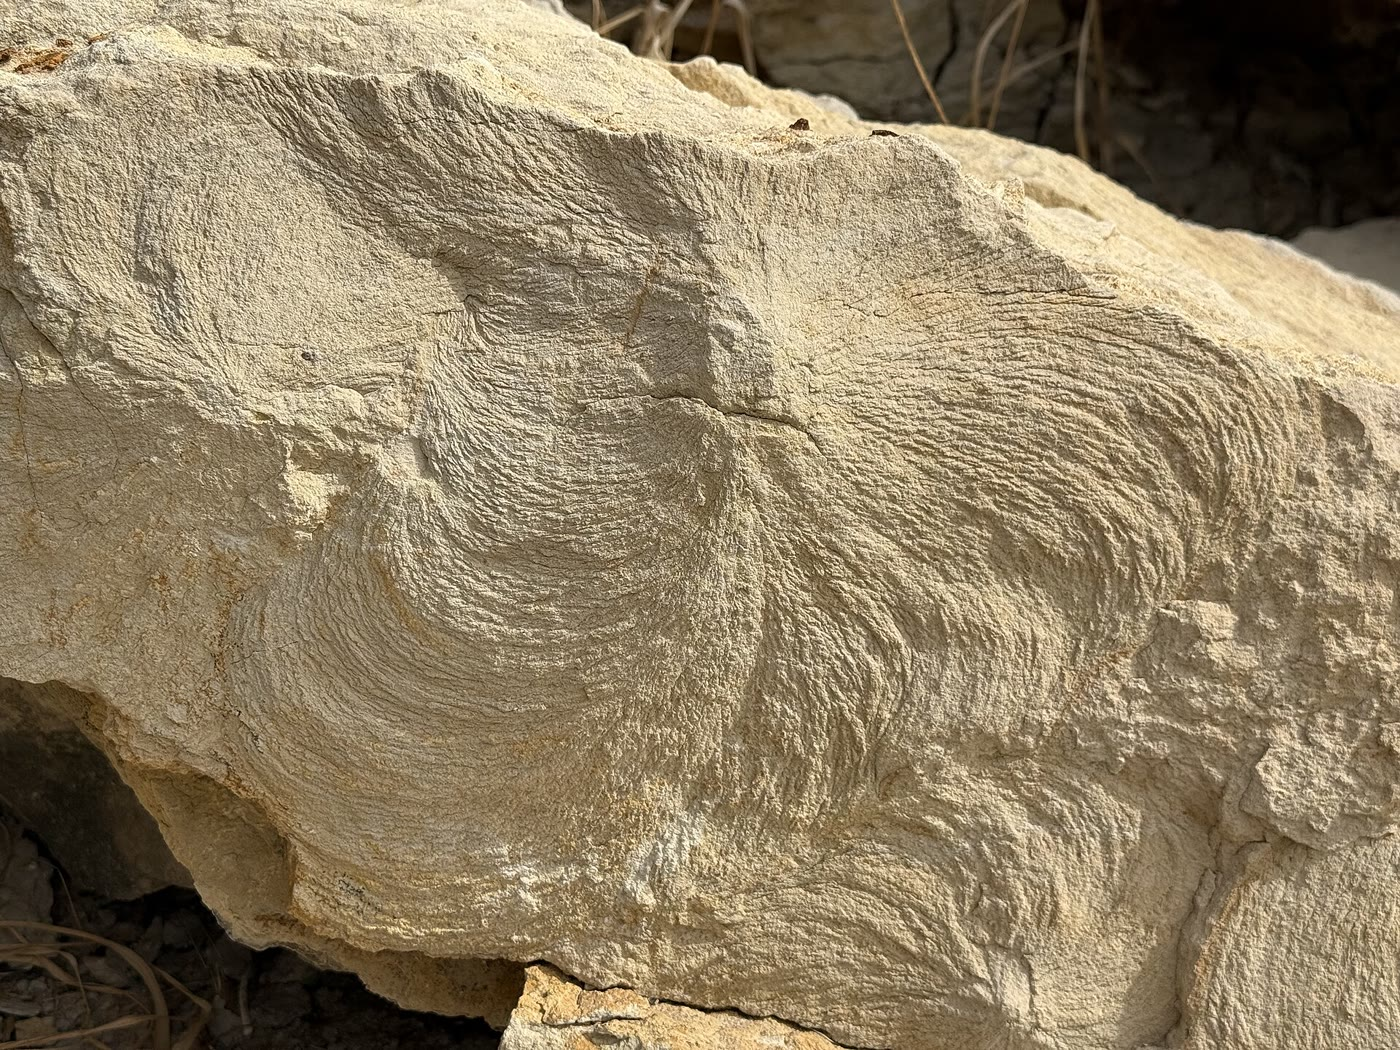
\includegraphics[width=0.5\linewidth]{images/book4/b2-20-zoophycos.jpg}
\par\smallskip{\small \emph{Zoophycos} en un bloque de Sagres, Portugal: los arcos son las lamelas
de una lámina helicoidal de sedimento removido. (Amada44, CC~BY~4.0, a través de Wikimedia Commons.)}
\end{omfigure}
% ledger: zhang15:zoophycos

\section{Leer un mar desaparecido}\label{sec:b2:palaeoenvironments:varden}

Los ambientes están uno junto a otro: una playa, un fondo de plataforma externa, una plataforma más profunda. Cuando el mar sube o
el fondo se hunde, cada ambiente se desplaza hacia tierra sobre su vecino, y sus depósitos pasan a quedar
encima de los del vecino. Una sucesión vertical de facies, sin interrupción, repite así
el orden de los ambientes que estaban uno al lado del otro; el volumen de tercer año hace de esta regla,
la ley de Walther, su punto de partida. Una columna leída de abajo arriba es una película de la costa desplazándose
sobre un lugar.

La cobertera de las colinas de Varden, la región inventada de la serie, ofrece un ejemplo completo. Sus
espesores son los del modelo de la región; los fósiles de la figura siguiente se han inventado para ella,
pero cada uno se ha elegido de modo que rocas reales de ese tipo puedan contenerlo. A la caliza se le asigna el
Toarciense, de 184.2 a \qty{174.7}{Ma}, y a la lutita del Aaleniense al Calloviense, de
\qty{174.7}{Ma} a \qty{161.5}{Ma}.
% ledger: data:b4-palaeoenv, ics4:jurassic-stages

\begin{omfigure}
\centering
% figdata/bachelor-2/palaeoenv.py part log (thicknesses from figdata/shared/region.py)
\begin{tikzpicture}[x=1cm, y=0.0165cm, font=\scriptsize]
% scale
\draw[black!70] (-0.35,0) -- (-0.35,460);
\foreach \z in {0,100,...,400} {\draw[black!70] (-0.45,\z) -- (-0.35,\z) node[left=3pt] {\z};}
\node[rotate=90, anchor=south] at (-1.15,230) {altura sobre la base de la cobertera (m)};
% units
\fill[lith sandstone] (0,0) rectangle (2.2,120);
\fill[lith limestone] (0,120) rectangle (2.0,180);
\fill[lith limestone] (0,180) rectangle (1.6,300);
\fill[lith shale] (0,300) rectangle (1.1,400);
\fill[om lith={icsCretaceous!35}{om limestone}] (0,400) -- (1.4,400) -- (1.4,452)
  .. controls (1.0,466) and (0.6,446) .. (0.3,458) -- (0,455) -- cycle;
\draw[black!70] (0,0) rectangle (2.2,120);
\draw[black!70] (0,120) rectangle (2.0,180);
\draw[black!70] (0,180) rectangle (1.6,300);
\draw[black!70] (0,300) rectangle (1.1,400);
\draw[black!70] (0,400) -- (1.4,400) -- (1.4,452) .. controls (1.0,466) and (0.6,446) ..
  (0.3,458) -- (0,455) -- cycle;
\node[anchor=west, font=\tiny] at (1.45,460) {techo erosionado};
% unit names
\node[anchor=west, align=left] at (2.6,60) {\textbf{arenisca}, \qty{120}{m}\\Triásico};
\node[anchor=west, align=left] at (2.6,150) {\textbf{caliza oolítica}, \qty{60}{m}\\Toarciense};
\node[anchor=west, align=left] at (2.6,240) {\textbf{caliza fina}, \qty{120}{m}\\Toarciense};
\node[anchor=west, align=left] at (2.6,350) {\textbf{lutita}, \qty{100}{m}\\Aaleniense--Calloviense};
\node[anchor=west, align=left] at (2.6,424) {\textbf{creta}\\Cretácico};
% content
\node[anchor=west, align=left, text width=6.9cm] at (6.3,60) {rellenos de canal con estratificación cruzada sobre bases
  erosivas; huellas de raíces; fragmentos vegetales; ningún fósil marino};
\node[anchor=west, align=left, text width=6.9cm] at (6.3,150) {ooides con estratificación cruzada; tubos verticales
  y madrigueras en U; fragmentos de concha desgastados};
\node[anchor=west, align=left, text width=6.9cm] at (6.3,240) {osículos de crinoides, braquiópodos,
  belemnites, ammonites; rastros de reptación y madrigueras de alimentación; capas de conchas rotas con bases
  netas};
\node[anchor=west, align=left, text width=6.9cm] at (6.3,350) {gris oscuro, laminada en algunos puntos;
  pirita; ammonites y bivalvos de concha fina; madrigueras helicoidales con spreite en las capas más claras};
\node[anchor=west, align=left, text width=6.9cm] at (6.3,424) {cocolitos; equinoideos, esponjas;
  nódulos de sílex; bioturbada en todo su espesor};
\foreach \z in {120,180,300,400} {\draw[black!25] (2.25,\z) -- (13.2,\z);}
\node[font=\scriptsize\bfseries, anchor=south west] at (2.6,462) {unidad y edad};
\node[font=\scriptsize\bfseries, anchor=south west] at (6.3,462) {qué contienen las capas};
\end{tikzpicture}
\par\smallskip{\small La cobertera de las colinas de Varden como columna, con el contenido de sus unidades. Los
espesores son los del modelo de la región, salvo la creta, cuyo techo erosionado se corta aquí
(\qty{766}{m} de espesor en el sinclinal del \cref{ex:b2:palaeoenvironments:shale}); la anchura de la columna crece con el tamaño de grano;
los fósiles y sus edades se han inventado para la región.}
\end{omfigure}
% ledger: data:b4-palaeoenv, ics4:jurassic-stages

\begin{example}[La base de la cobertera de Varden]\label{ex:b2:palaeoenvironments:base}
La arenisca contiene rellenos de canal sobre bases erosivas, raíces y fragmentos vegetales, y ningún fósil
marino: la depositaron ríos en tierra firme. La caliza oolítica de encima tiene ooides con estratificación cruzada,
que crecen al rodar en aguas agitadas, tubos verticales y madrigueras en U de la \omterm{def:b2:palaeoenvironments:ichnofacies}{icnofacies} de Skolithos,
y fragmentos de concha desgastados, todos \omterm{def:b2:palaeoenvironments:assemblages}{alóctonos}: un bajío de la playa sumergida,
barrido por el oleaje. Entre ambas llegó el mar: el contacto registra una \omterm{def:b2:phanerozoic-earth:transgression}{transgresión marina}. En
el orden de la ley de Walther, a la llanura fluvial le siguió la orilla, y después el bajío.
\end{example}
% ledger: buatois20:ichnofacies

\subsection*{¿A qué velocidad se rellenó el fondo marino?}

Una biozona da una duración, una columna da un espesor, y su cociente es una velocidad. Pero el
espesor ha disminuido desde que se depositó el sedimento: el agua de los poros ha sido expulsada,
y solo se conservan los granos.

\begin{proposition}[Velocidad de acumulación de una capa compactada]\label{prop:b2:palaeoenvironments:rate}
Una capa de espesor actual $h$ y porosidad media $\varphi$, depositada durante el tiempo $\Delta t$
con la porosidad $\varphi_0$, se acumuló a la velocidad
\[
  r = \frac{h\,(1 - \varphi)}{(1 - \varphi_0)\,\Delta t}
\]
de sedimento fresco, y a la velocidad $h(1-\varphi)/\Delta t$ de granos, que no depende de
$\varphi_0$.
\end{proposition}

\begin{proof}
Por unidad de área, la capa contiene el volumen de granos $h(1 - \varphi)$, el espesor sólido del
volumen de primer año. La compactación expulsa agua pero no añade ni quita granos, así que el sedimento
fresco, de porosidad $\varphi_0$, tenía el espesor $h_0$ con $h_0(1 - \varphi_0) = h(1 -
\varphi)$. Dividiendo $h_0$ y el espesor sólido por $\Delta t$ se obtienen las dos velocidades.
\end{proof}

Cuando no se midió la porosidad, la ley de Athy la da a partir de la profundidad. La figura siguiente muestra
la ley para cuatro litologías, y el factor $(1 - \varphi(z))/(1 - \varphi_0)$ por el que hay que estirar una capa
delgada situada hoy a la profundidad $z$ para obtener su espesor en superficie. La creta y la lutita
empiezan con mucha agua y la pierden deprisa: una capa delgada de lutita a \qty{1000}{m} era 1.68 veces
más gruesa cuando se depositó, y una capa de creta, 2.19 veces.
% ledger: pybacktrack:compaction, pybacktrack4:limestone, data:b4-palaeoenv

\begin{omfigure}
\centering
% figdata/bachelor-2/palaeoenv.py parts poro and ratio
\begin{tikzpicture}
\begin{groupplot}[group style={group size=2 by 1, horizontal sep=1.6cm},
  width=0.46\linewidth, height=6.2cm, y dir=reverse, ymin=0, ymax=3000,
  tick label style={font=\scriptsize}, label style={font=\small}, xtick pos=bottom,
  ytick pos=left, scaled y ticks=false, yticklabel style={/pgf/number format/1000 sep={\,}}]
\nextgroupplot[xmin=0, xmax=0.75, xlabel={porosidad $\varphi$}, ylabel={profundidad $z$ (\unit{m})},
  legend style={at={(0.5,1.04)}, anchor=south, draw=none, font=\scriptsize, legend columns=2}]
\addplot[omThm, line width=1pt] table[x=shale, y=z_m] {figdata/out/bachelor-2-palaeoenv-poro.dat};
\addlegendentry{lutita}
\addplot[omSea!80!black, line width=1pt, dashed] table[x=sandstone, y=z_m] {figdata/out/bachelor-2-palaeoenv-poro.dat};
\addlegendentry{arenisca}
\addplot[black, line width=1pt, dotted] table[x=chalk, y=z_m] {figdata/out/bachelor-2-palaeoenv-poro.dat};
\addlegendentry{creta}
\addplot[green!45!black, line width=1pt, dash dot] table[x=limestone, y=z_m] {figdata/out/bachelor-2-palaeoenv-poro.dat};
\addlegendentry{caliza}
\nextgroupplot[xmin=1, xmax=3.2, xlabel={factor de restauración $(1-\varphi)/(1-\varphi_0)$}]
\addplot[omThm, line width=1pt] table[x=shale, y=z_m] {figdata/out/bachelor-2-palaeoenv-ratio.dat};
\addplot[omSea!80!black, line width=1pt, dashed] table[x=sandstone, y=z_m] {figdata/out/bachelor-2-palaeoenv-ratio.dat};
\addplot[black, line width=1pt, dotted] table[x=chalk, y=z_m] {figdata/out/bachelor-2-palaeoenv-ratio.dat};
\addplot[green!45!black, line width=1pt, dash dot] table[x=limestone, y=z_m] {figdata/out/bachelor-2-palaeoenv-ratio.dat};
\end{groupplot}
\end{tikzpicture}
\par\smallskip{\small Izquierda: porosidad en función de la profundidad según la ley de Athy, con las constantes de Sclater
y Christie (1980) para la lutita, la arenisca y la creta y de Turer y Maynard (2003) para la caliza,
tal como las tabula pyBacktrack. Derecha: el factor por el que una capa delgada a la profundidad $z$ se
restaura a su espesor en superficie.}
\end{omfigure}
% ledger: pybacktrack:compaction, pybacktrack4:limestone, data:b4-palaeoenv

\begin{example}[La lutita de Varden]\label{ex:b2:palaeoenvironments:shale}
En el sinclinal de las colinas de Varden la creta tiene \qty{766}{m} de espesor, así que la lutita está entre
766 y \qty{866}{m}. Con las constantes de la lutita, $\varphi_0 = 0.63$ y $\lambda =
\qty{1960}{m}$, el espesor sólido del volumen de primer año es $100 - 0.63 \times 1960 \times
(e^{-766/1960} - e^{-866/1960}) = \qty{58.4}{m}$, una porosidad media de 0.416. Devuelta a la
superficie con los mismos granos, la capa tiene \qty{148.6}{m} de espesor. En los \qty{13.2}{Myr} que van desde
la base del Aaleniense hasta el techo del Calloviense, la lutita se acumuló a $100/13.2 =
\qty{7.6}{m}$ por millón de años tal como está hoy, a $148.6/13.2 = \qty{11.3}{m}$ por millón de
años de fango fresco, y a \qty{4.4}{m} por millón de años de granos. El espesor actual
infravalora la velocidad en un tercio.
\end{example}
% ledger: data:b4-palaeoenv, pybacktrack:compaction, ics4:jurassic-stages

La lutita pudo estar en otro tiempo aún más profunda, bajo una creta erosionada después; la corrección es entonces un
mínimo. El problema de fin de semana aplica la proposición a la caliza, cuya porosidad se
midió.

\section*{Ejercicios}\label{sec:b2:palaeoenvironments:exercises}

Datos para los ejercicios, salvo indicación contraria: ley de Athy $\varphi = \varphi_0 e^{-z/\lambda}$
con $\varphi_0 = 0.63$, $\lambda = \qty{1960}{m}$ (lutita), $0.49$, \qty{3704}{m} (arenisca),
$0.70$, \qty{1408}{m} (creta), $0.51$, \qty{4545}{m} (caliza); calcita \qty{2710}{kg.m^{-3}},
agua intersticial \qty{1000}{kg.m^{-3}}; las edades de la tabla internacional: Toarciense de 184.2 a
\qty{174.7}{Ma}.
% ledger: pybacktrack:compaction, pybacktrack4:limestone, ics4:jurassic-stages

\begin{exercise}[$\star$]\label{exo:b2:palaeoenvironments:1}
En 51 estaciones de un fondo costero se encontraron vivas 135 especies de invertebrados, 150 entre las conchas
y los esqueletos muertos del fondo, y 112 que tienen además registro fósil. (a) Exprésese el tercer
número como fracción de cada uno de los dos primeros. (b) ¿Cómo pueden los muertos superar a los vivos? (c)
¿Qué grupos tróficos esperaría usted que estuvieran infrarrepresentados entre los muertos, y por qué?
\end{exercise}
% ledger: tyler25:live-dead, tyler25:soft-bodied

\begin{exercise}[$\star$]\label{exo:b2:palaeoenvironments:2}
Un horizonte de ammonites del Jurásico Superior dura en promedio \qty{165}{kyr}. (a) ¿Cuánto duran cinco horizontes?
Compárese con los 0.7 a 1 millón de años dados para \emph{Archaeopteryx}. (b) La primera
zona del Toarciense abarca de 183.73 a \qty{182.77}{Ma}: ¿cuántos horizontes de duración media contendría?
(c) ¿Por qué importan los horizontes, y no las zonas, para seguir la evolución de un linaje?
\end{exercise}
% ledger: rauhut18:archaeopteryx, alsuwaidi22:toarcian

\begin{exercise}[$\star$]\label{exo:b2:palaeoenvironments:3}
Nómbrense la \omterm{def:b2:palaeoenvironments:ichnofacies}{icnofacies} y el marco de cada conjunto. (a) Rastros de ramoneo en meandros y redes regulares de
madrigueras en las bases de turbiditas delgadas. (b) Tubos verticales muy juntos en arena limpia con
estratificación cruzada. (c) Abundantes madrigueras horizontales de sedimentívoros y huellas de ramoneo en capas
limosas entre arenas de tormenta. (d) Madrigueras helicoidales con spreite en un fango fino y oscuro sin ondulaciones
de oleaje, en rocas mesozoicas.
\end{exercise}
% ledger: buatois20:ichnofacies, paz23:nereites

\begin{exercise}[$\star$]\label{exo:b2:palaeoenvironments:4}
La capa A contiene crinoides, braquiópodos, corales y trilobites; la capa B, de la misma edad, contiene restos
vegetales, huesos de peces, unos pocos bivalvos y gasterópodos, y numerosos individuos de solo dos especies de
ostrácodos. (a) ¿Qué dice cada una sobre la salinidad de su agua? (b) A la capa B le faltan los grupos de
la capa A: ¿por qué esa ausencia es un argumento, mientras que la ausencia de un fósil en una capa no lo es?
(c) ¿Qué otras observaciones pondrían a prueba la interpretación de la capa B?
\end{exercise}
% ledger: mcgairy21:stenohaline, saleh22:echinoderms

\begin{exercise}[$\star\star$]\label{exo:b2:palaeoenvironments:5}
Úsese la \cref{prop:b2:palaeoenvironments:burial} con la concha del
\cref{ex:b2:palaeoenvironments:shell}, $k = \qty{0.05}{yr^{-1}}$ y $h = \qty{0.1}{m}$. (a)
Hállese la velocidad de sedimentación con la que la mitad de las conchas llegan a estar a salvo. (b) ¿En qué factor
cambia $P$ cuando la velocidad se reduce a la mitad de ese valor? (c) Una concha el doble de gruesa sobrevive el doble de tiempo
en el fondo. Con \qty{1}{mm.yr^{-1}}, ¿cuánto más probable es que se conserve? (d) ¿Qué implica
esto para las proporciones de conchas finas y gruesas en una asociación fósil?
\end{exercise}
% ledger: tyler25:soft-bodied

\begin{exercise}[$\star\star$]\label{exo:b2:palaeoenvironments:6}
Las capas de ceniza datan la base del Toarciense en Chacay Melehue en $183.73$, $+0.35$, \qty{-0.50}{Myr};
la tabla internacional da \qty{184.2}{Ma}. (a) ¿Está el valor de la tabla dentro de la incertidumbre?
¿Por cuánto se sale de la cota superior? (b) La primera zona del Toarciense termina a
\qty{182.77}{Ma}: hállese su duración. (c) Supóngase que esta zona tiene \qty{6}{m} de espesor en una sección:
¿cuál es la velocidad de acumulación? (d) ¿Por qué una biozona puede ser la misma en todas partes en el tiempo mientras su
espesor varía de un lugar a otro?
\end{exercise}
% ledger: alsuwaidi22:toarcian, ics4:jurassic-stages

\begin{exercise}[$\star\star$]\label{exo:b2:palaeoenvironments:7}
En el sinclinal de Varden la arenisca está entre 1046 y \qty{1166}{m} bajo el suelo. (a)
Hállense su porosidad según la ley de Athy en el techo y en la base, y su porosidad media, redondeada a
tres decimales, a partir del promedio de ambas. (b) Hállese su espesor sólido. (c) Restáurese a la
superficie con el factor de capa delgada a la porosidad media. (d) La restauración exacta da
\qty{147.0}{m}. ¿Por qué la estimación de capa delgada es algo demasiado grande?
\end{exercise}
% ledger: data:b4-palaeoenv, pybacktrack:compaction

\begin{exercise}[$\star\star$]\label{exo:b2:palaeoenvironments:8}
Un registro de densidad marca \qty{2573}{kg.m^{-3}} en la caliza de Varden, formada por granos de calcita con
agua en los poros. (a) Demuéstrese que la porosidad es $\varphi = (\rho_{\text{grano}} -
\rho)/(\rho_{\text{grano}} - \rho_{\text{agua}})$ y calcúlese. (b) A la profundidad media de la
caliza en el sinclinal, \qty{956}{m}, ¿qué predice la ley de Athy con las constantes de la caliza?
(c) ¿Qué proceso diagenético puede explicar la diferencia?
\end{exercise}
% ledger: pybacktrack4:limestone, data:b4-palaeoenv

\begin{exercise}[$\star\star$]\label{exo:b2:palaeoenvironments:9}
Un acantilado de rocas jurásicas muestra de la base hacia arriba: turbiditas delgadas con meandros regulares y redes de
madrigueras; fango oscuro con madrigueras helicoidales con spreite; capas limosas con madrigueras de sedimentívoros entre
arenas de tormenta; arena limpia con estratificación cruzada y
tubos verticales; después, un carbón con raíces. (a) Interprétese cada parte. (b) ¿Se hizo el agua más profunda o más
somera? (c) Nómbrense dos causas que podrían producir esta sucesión, y dígase qué permitiría decidir
entre ellas. (d) ¿Por qué un salto brusco de la primera parte a la cuarta, sin las demás, es una
advertencia?
\end{exercise}
% ledger: buatois20:ichnofacies, paz23:nereites

\begin{exercise}[$\star\star\star$]\label{exo:b2:palaeoenvironments:10}
Un animal de cuerpo blando sobrevive en el fondo un año de media ($k = \qty{1}{yr^{-1}}$), y una
concha, un siglo; ambos están a salvo bajo $h = \qty{0.1}{m}$. (a) Compárense sus probabilidades de
preservación a 1, 10 y \qty{100}{mm.yr^{-1}}. (b) Hállese la velocidad con la que se conserva un cuerpo blando de cada
cien. (c) ¿Es plausible una velocidad así durante meses seguidos? ¿Qué clase de depósito entierra
el fondo más deprisa? (d) ¿Qué hipótesis de la \cref{prop:b2:palaeoenvironments:burial} falla para un
depósito así, y cómo se comporta la fórmula cuando falla?
\end{exercise}

\begin{exercise}[$\star\star\star$]\label{exo:b2:palaeoenvironments:11}
(a) Demuéstrese que el factor de capa delgada $(1 - \varphi(z))/(1 - \varphi_0)$ se deduce de la
\cref{prop:b2:palaeoenvironments:rate}. (b) Aplíquese a la profundidad media de la lutita de Varden,
\qty{816}{m}, para restaurar los \qty{100}{m} de lutita. (c) Compárese con los \qty{148.6}{m} exactos del
\cref{ex:b2:palaeoenvironments:shale}, y explíquese el signo de la diferencia. (d) Demuéstrese que la
velocidad de granos, a diferencia de la velocidad de sedimento fresco, puede compararse entre una lutita y una caliza
sin saber lo porosa que era cada una al depositarse.
\end{exercise}
% ledger: data:b4-palaeoenv, pybacktrack:compaction

\begin{exercise}[$\star\star\star$]\label{exo:b2:palaeoenvironments:12}
Supóngase que los horizontes de ammonites del Toarciense duran \qty{165}{kyr} en promedio, como los del Jurásico Superior.
(a) ¿Cuántos horizontes contendrían los \qty{180}{m} de la caliza de Varden? (b) ¿Qué espesor de
caliza representa hoy un horizonte, y qué espesor de sedimento fresco, sabiendo que la
capa tenía \qty{338}{m} de espesor al depositarse? (c) Para estar seguro de encontrar todos los horizontes, un
geólogo muestrea a no más de la mitad de ese espesor actual: ¿qué espaciado es ese, y cuántas
muestras? (d) ¿Por qué podrían faltar algunos horizontes aun así?
\end{exercise}
% ledger: rauhut18:archaeopteryx, ics4:jurassic-stages, data:b4-palaeoenv

\begin{problem}[{Problema de fin de semana --- El mar jurásico de las colinas de Varden}]\label{pb:b2:palaeoenvironments:1}
Este problema lee el ambiente y la historia de la cobertera de Varden, con la columna de la
\cref{sec:b2:palaeoenvironments:varden} y los datos de los ejercicios. La cobertera buza
\ang{12} en los flancos de los pliegues; en el sinclinal la atraviesa un sondeo.

\medskip\noindent\textbf{Parte I --- Las rocas y su espesor.}
\begin{enumerate}
  \item En terreno llano sobre un flanco, la caliza aflora en una anchura de \qty{866}{m}, medida
        perpendicularmente a la dirección. Hállese su espesor real.
  \item La lutita aflora en \qty{481}{m}. Hállese su espesor.
  \item ¿Qué unidad es la más antigua, y según qué principio?
  \item En el sondeo, la lutita empieza a \qty{766}{m}, la caliza a \qty{866}{m} y la
        arenisca a \qty{1046}{m} bajo el suelo. Compruébense los espesores.
  \item La creta está cortada por la superficie del terreno. ¿Qué puede decirse de su espesor cuando
        se retiró el mar cretácico?
  \item Hállese la porosidad de la creta en la superficie y en la base de la creta en el sondeo.
\end{enumerate}

\medskip\noindent\textbf{Parte II --- Ambientes.}
\begin{enumerate}[resume]
  \item ¿Qué dicen los crinoides, braquiópodos, belemnites y ammonites de la caliza fina
        sobre su agua?
  \item ¿Qué \omterm{def:b2:palaeoenvironments:ichnofacies}{icnofacies} forman sus huellas, y en qué parte del perfil?
  \item ¿Qué registran sus capas de conchas rotas con bases netas?
  \item La lutita es oscura, laminada en algunos puntos, con pirita y pocas madrigueras. ¿Qué dice eso
        sobre el agua del fondo?
  \item Sus capas más claras contienen madrigueras helicoidales con spreite. ¿Qué \omterm{def:b2:palaeoenvironments:ichnofacies}{icnofacies}, y qué marco?
  \item ¿Forman los ammonites de la lutita parte de una \omterm{def:b2:palaeoenvironments:assemblages}{asociación de vida} del fondo? Explíquese.
\end{enumerate}

\medskip\noindent\textbf{Parte III --- Tiempo y velocidades.} Las capas más bajas de la caliza contienen los
ammonites de la primera zona del Toarciense, las más altas los de la última, y la lutita empieza con
la primera zona del Aaleniense.
\begin{enumerate}[resume]
  \item ¿Cuánto tardó en acumularse la caliza?
  \item ¿A qué velocidad, tal como está hoy la caliza?
  \item El registro de densidad del sondeo marca \qty{2573}{kg.m^{-3}} en la caliza. Hállese su
        porosidad.
  \item El fango calcáreo se deposita con una porosidad de 0.51. Hállese el espesor del sedimento fresco.
  \item Hállese la velocidad de sedimento fresco.
  \item Hállese la velocidad de granos.
  \item Compárese con la lutita del \cref{ex:b2:palaeoenvironments:shale}. ¿Qué sugiere el cambio de
        velocidad sobre el aporte de carbonato?
\end{enumerate}

\medskip\noindent\textbf{Parte IV --- El mar sobre Varden.}
\begin{enumerate}[resume]
  \item Léase la columna de la arenisca a la creta. ¿Avanzó o retrocedió el mar?
  \item En la curva a largo plazo de Haq y otros, el nivel del mar global estaba unos 41, 57 y
        \qty{86}{m} por encima del actual a 184, 174 y \qty{162}{Ma}. ¿Cuánto subió durante la
        caliza, durante la lutita, y en total?
  \item Supóngase que el fondo pasó de \qty{5}{m} de agua en el bajío a \qty{60}{m} en el techo de
        la lutita. Hállese el espacio de acomodación creado desde la base de la caliza hasta el techo de la
        lutita, contando los espesores frescos de ambas unidades, y su velocidad media.
  \item ¿Qué parte puede explicar la subida global? ¿Qué produjo el resto?
  \item En resumen: ¿a qué velocidad se acumuló el fango calcáreo de la caliza de Varden cuando se
        depositó?
\end{enumerate}
\end{problem}
% ledger: data:b4-palaeoenv, ics4:jurassic-stages, pybacktrack4:limestone, pybacktrack:compaction, data:b4-sealevel, haq87:charts, buatois20:ichnofacies, mcgairy21:stenohaline
